	\chapter*{Dodatak: Prikaz aktivnosti grupe}
		\addcontentsline{toc}{chapter}{Dodatak: Prikaz aktivnosti grupe}
		
		\section*{Dnevnik sastajanja}

		\begin{packed_enum}
			\item  sastanak
			
			\item[] \begin{packed_item}
				\item Datum: u ovom formatu: 16.listopada 2023.
				\item Prisustvovali: H.Ivančić, D.Ljubić, I.Pavlović, M.Perković, D.Petrović, K.Raštegorac, F.Širić
				\item Teme sastanka:
				\begin{packed_item}
					\item  upoznavanje s temom
				\end{packed_item}
			\end{packed_item}
			
			\item  sastanak
			\item[] \begin{packed_item}
				\item Datum: u ovom formatu: 25.listopada 2023.
				\item Prisustvovali: H.Ivančić, I.Pavlović, M.Perković, D.Petrović, K.Raštegorac, F.Širić
				\item Teme sastanka:
				\begin{packed_item}
					\item  raspodjela posla
					\item  početak rada
				\end{packed_item}
			\end{packed_item}
			
			\item  sastanak
			\item[] \begin{packed_item}
				\item Datum: 2.studenoga 2023.
				\item Prisustvovali: H.Ivančić, D.Ljubić, I.Pavlović, M.Perković, D.Petrović, K.Raštegorac, F.Širić
				\item Teme sastanka:
				\begin{packed_item}
					\item  provjera dotad završene dokumentacije
					\item detaljnija raspodjela posla
				\end{packed_item}
			\end{packed_item}
			
			\item  sastanak
			\item[] \begin{packed_item}
				\item Datum: 9.studenoga 2023.
				\item Prisustvovali: H.Ivančić, D.Ljubić, I.Pavlović, M.Perković, D.Petrović, K.Raštegorac, F.Širić
				\item Teme sastanka:
				\begin{packed_item}
					\item  testiranje dotad dovršene implementacije
					\item  provjera dotad završene dokumentacije
				\end{packed_item}
			\end{packed_item}
			
			\item  sastanak
			\item[] \begin{packed_item}
				\item Datum: 17.studenoga 2023.
				\item Prisustvovali: H.Ivančić, D.Ljubić, I.Pavlović, M.Perković, D.Petrović, K.Raštegorac, F.Širić
				\item Teme sastanka:
				\begin{packed_item}
					\item  posljednja provjera ispravnosti dokumentacije
					\item  posljednja provjera implementacije funkcionalnosti
				\end{packed_item}
			\end{packed_item}
			
			\item  sastanak
			\item[] \begin{packed_item}
				\item Datum: 11.prosinca 2023.
				\item Prisustvovali: H.Ivančić, D.Ljubić, I.Pavlović, M.Perković, D.Petrović, K.Raštegorac, F.Širić
				\item Teme sastanka:
				\begin{packed_item}
					\item  dogovor o daljnjem tijeku rada
					\item zadavanje ciljeva implementacije za 2. ciklus
				\end{packed_item}
			\end{packed_item}
			
			\item  sastanak
						\item[] \begin{packed_item}
				\item Datum: 18.prosinca 2023.
				\item Prisustvovali: H.Ivančić, D.Ljubić, I.Pavlović, M.Perković, D.Petrović, K.Raštegorac, F.Širić
				\item Teme sastanka:
				\begin{packed_item}
					\item statusni sastanak
					\item plan daljnjeg rada
				\end{packed_item}
			\end{packed_item}
			
			\item  sastanak
			\begin{packed_item}
				\item Datum: 29.prosinca 2023.
				\item Prisustvovali: H.Ivančić, D.Ljubić, M.Perković, K.Raštegorac, F.Širić
				\item Teme sastanka:
				\begin{packed_item}
					\item dogovor o dijelovima frontend aplikacije
				\end{packed_item}
			\end{packed_item}
			
						\item  sastanak
						\begin{packed_item}
				\item Datum: 5.siječnja 2024.
				\item Prisustvovali: H.Ivančić, D.Ljubić, I.Pavlović, M.Perković, D.Petrović, K.Raštegorac, F.Širić
				\item Teme sastanka:
				\begin{packed_item}
					\item statusni sastanak
					\item konzultacije o izradi preostalog dijela dokumentacije
				\end{packed_item}
			\end{packed_item}
			
					\item sastanak				\begin{packed_item}
				\item Datum: 12.siječnja 2024.
				\item Prisustvovali: H.Ivančić, D.Ljubić, I.Pavlović, M.Perković, D.Petrović, K.Raštegorac, F.Širić
				\item Teme sastanka:
				\begin{packed_item}
					\item briefing dotad implementiranog
					\item posljednje izmjene baze podataka
				\end{packed_item}
			\end{packed_item}
			
						\item  sastanak
		\begin{packed_item}
				\item Datum: 13.siječnja 2024.
				\item Prisustvovali: H.Ivančić, D.Ljubić, I.Pavlović, M.Perković, D.Petrović, K.Raštegorac, F.Širić
				\item Teme sastanka:
				\begin{packed_item}
					\item briefing dotad implementiranog
					\item posljednje izmjene baze podataka
				\end{packed_item}
			\end{packed_item}
			
						\item  sastanak
					\begin{packed_item}
				\item Datum: 16.siječnja 2024.
				\item Prisustvovali: H.Ivančić, D.Ljubić, I.Pavlović, M.Perković, D.Petrović, K.Raštegorac, F.Širić
				\item Teme sastanka:
				\begin{packed_item}
					\item briefing dotad implementiranog
				\end{packed_item}
			\end{packed_item}
			
						\item  sastanak					\begin{packed_item}
				\item Datum: 19.siječnja 2024.
				\item Prisustvovali: H.Ivančić, D.Ljubić, I.Pavlović, M.Perković, D.Petrović, K.Raštegorac, F.Širić
				\item Teme sastanka:
				\begin{packed_item}
					\item posljednje izmjene dokumentacije
					\item posljednja provjera inmplementacije
				\end{packed_item}
			\end{packed_item}
			
			
			
			%
			
		\end{packed_enum}
		
		\eject
		\section*{Tablica aktivnosti}
		
			\textbf{\textit{Kontinuirano osvježavanje}}\\
			
			 \textit{Napomena: Doprinose u aktivnostima treba navesti u satima po članovima grupe po aktivnosti.}

			\begin{longtblr}[
					label=none,
				]{
					vlines,hlines,
					width = \textwidth,
					colspec={X[7, l]X[1, c]X[1, c]X[1, c]X[1, c]X[1, c]X[1, c]X[1, c]}, 
					vline{1} = {1}{text=\clap{}},
					hline{1} = {1}{text=\clap{}},
					rowhead = 1,
				} 
			
				\SetCell[c=1]{c}{} & \SetCell[c=1]{c}{\rotatebox{90}{\textbf{Hana Ivančić}}} & \SetCell[c=1]{c}{\rotatebox{90}{\textbf{David Ljubić}}} &	\SetCell[c=1]{c}{\rotatebox{90}{\textbf{Ivan Pavlović}}} & \SetCell[c=1]{c}{\rotatebox{90}{\textbf{Marija Perković}}} &	\SetCell[c=1]{c}{\rotatebox{90}{\textbf{Dunja Petrović}}} & \SetCell[c=1]{c}{\rotatebox{90}{\textbf{Karlo Raštegorac}}} &	\SetCell[c=1]{c}{\rotatebox{90}{\textbf{Fran Širić}}} \\  
				Upravljanje projektom 		& 20 &  1&  &  &  2&  & \\ 
				Opis projektnog zadatka 	&  &  &  &  &  4&  & \\ 
				
				Funkcionalni zahtjevi       & 3 &  &  &  & 7 &  &  \\ 
				Opis pojedinih obrazaca 	&  1&  &  &  & 5 &  &  \\ 
				Dijagram obrazaca 			& 6 &  &  &  & 2 &  &  \\ 
				Sekvencijski dijagrami 		&  5&  &  &  & 2 &  &  \\ 
				Opis ostalih zahtjeva 		&  &  &  &  & 1 &  &  \\ 

				Arhitektura i dizajn sustava	 &  &  &  &  &8  &  &  \\ 
				Baza podataka				&  &  &  &  &  8&  &   \\ 
				Dijagram razreda 			& 6 &  &  &  &  4&  &   \\ 
				Dijagram stanja				&  &  &  &  & 3 &  &  \\ 
				Dijagram aktivnosti 		&  &  &  &  &  3&  &  \\ 
				Dijagram komponenti			&  &  &  &  &3  &  &  \\ 
				Korištene tehnologije i alati 		& 5 & 2  & 2 & 2 & 2 & 2 & 5 \\ 
				Ispitivanje programskog rješenja 	& 10 & 10 &  & 10 & 5 & 10  & 10 \\ 
				Dijagram razmještaja			&  &  &  &  & 2 &  &  \\ 
				Upute za puštanje u pogon 		&  &  &  &  &2  &  &  \\  
				Dnevnik sastajanja 			&  &  &  &  & 1 &  &  \\ 
				Zaključak i budući rad 		&  &  &  &  & 1 &  &  \\  
				Popis literature 			&  &  &  &  & 2 &  &  \\  
				&  &  &  &  &  &  &  \\ \hline 
				\textit{Dodatne stavke kako ste podijelili izradu aplikacije} 			&  &  &  &  &  &  &  \\ 
				\textit{izrada baze podataka} 		 			&  &  & 17 &  &  &  & 5\\  
				\textit{spajanje s bazom podataka} 							&  &  & 2 &  &  &  & 2 \\ 
				\textit{back end} 							&  &  &  &  &  &  & 30 \\ 
				\textit{komponenta za odabir recepta} 							&  &  &  &  &  &  20& \\ 
				\textit{komponenta za pregled entuzijasta} 							&  &  &  & 20 &  &  & \\ 
				\textit{početna stranica za neregistririane i registrirane korisnike} 							&  15&  &  &  & 1 &  & \\ 
				\textit{komponente za kuharice i recepte} 							& 3 &  &  & 6 &  &  & \\ 
				\textit{komponenta za uređivanje profila} 							&  &  5 &  &  &  &  &  \\ 
				\textit{komponenta za nutricionista} 							&  & 20 &  &  &  &  & \\ 
				\textit{dohvat podataka iz baze i proslijeđivanje fron endu} 							&  &  & 2 &  &  &  & 40\\ 
				\textit{obrada slika} 							&  & & 1 &  &  &  & \\ 
				\textit{deploy} 							& 12  & 1 & 1 & 1 & 1 & 1 & 1 \\ 
				\textit{JUnit testovi} 							&  & &  &  & 10 &  & \\  
			\end{longtblr}
			
			\section*{Dijagrami pregleda promjena}
			
			
			\begin{figure}[H]
			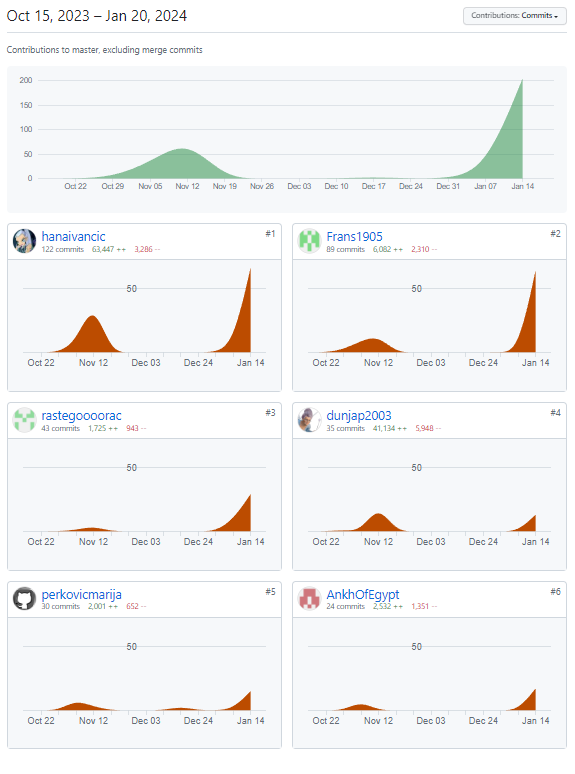
\includegraphics[scale=1.0]{slike/githubAktivnost.png} %veličina slike u odnosu na originalnu datoteku i pozicija slike
			\centering
			\caption{prikaz aktivnosti na repozitoriju}
			\label{prikaz aktivnosti na repozitoriju}
		\end{figure}
		
		\eject